\documentclass[12pt]{article}
\usepackage{graphicx, pst-func, pstricks, subfigure}% to put in axodraw

\begin{document}
\begin{figure}
	\subfigure[FDoG Kernel] {
		\psset{unit=1}
		\begin{pspicture}(0,0)(2,2)
			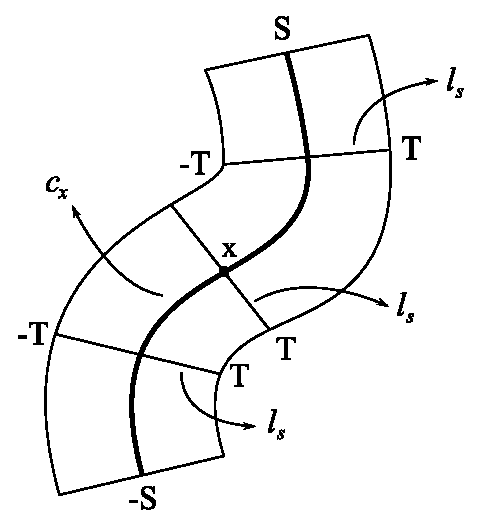
\includegraphics[width=2in]{pictures/fdog_kernel.eps}
		\end{pspicture}
	}
	\subfigure[Gaussian components for DoG] {
		\psset{unit=2}
		\begin{pspicture}(-2,-0.5)(2,2) 
			\psaxes[labels=none,ticks=none]{}(0,0)(-1.5,0)(1.5,1.5)
			\rput(-1,-0.2){\textit{-T}}
			\rput(1,-0.2){\textit{T}}
			\rput(0,-0.2){0}
			\psGauss[linecolor=red, linewidth=1pt, sigma=0.5]{-1.5}{1.5}
			\psGauss[linecolor=blue, linewidth=1pt, sigma=0.3125]{-1}{1}
			\psline{->}(0.5,1.7)(0.2,1.2)
			\rput(0.6,1.8){$G_{\sigma_{c}}$}
			\psline{->}(1.2,0.7)(0.9,0.2)
			\rput(1.3,0.8){$G_{\sigma_{s}}$}
		\end{pspicture}
	}	
\end{figure}



\end{document}
